\documentclass[tikz,border=1.35mm]{standalone}

\definecolor{fvmadaptedge}{HTML}{8A7E7E}
\usetikzlibrary{arrows.meta}

\definecolor{splitred}{HTML}{AF2525}

% Pentagonal face before and after isotropic face splitting.
% Coordinates are in millimeters; y=-1mm keeps the SVG-style origin at top left.
\begin{document}
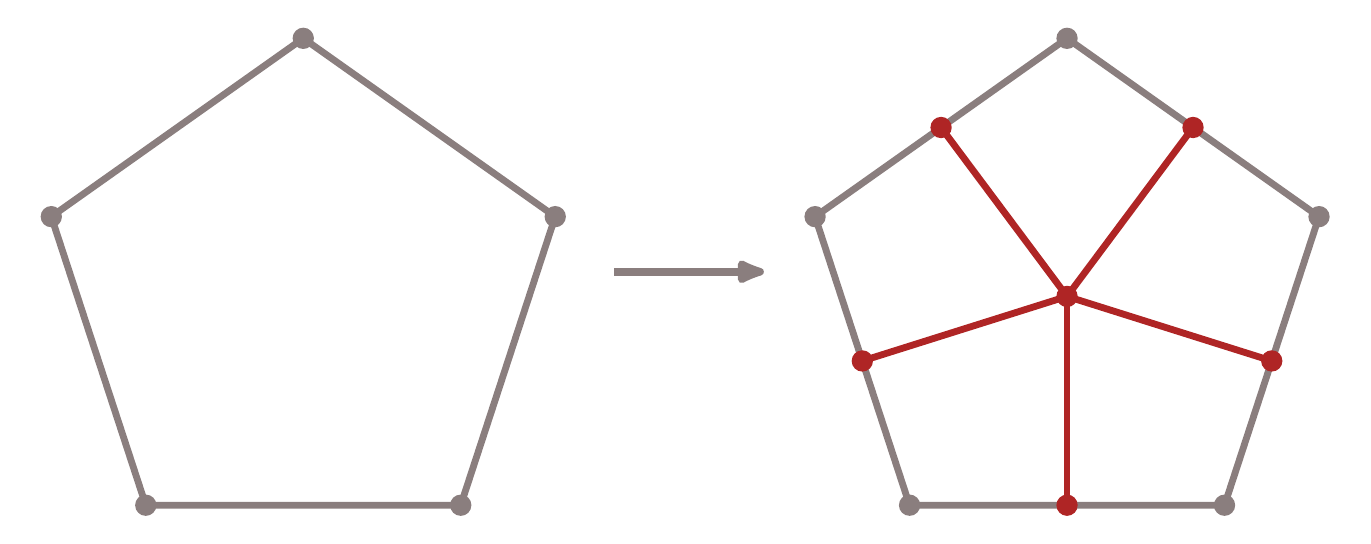
\begin{tikzpicture}[
  x=1mm,
  y=-1mm,
  line join=round,
  edge/.style={draw=fvmadaptedge,line width=0.865mm},
  splitline/.style={draw=splitred,line width=0.865mm},
  arrow/.style={draw=fvmadaptedge,line width=1.05mm,-{Latex[round,length=4.8mm,width=3.6mm]}}
]
  % Match the artwork frame before the standalone border is applied.
  \useasboundingbox (0,0) rectangle (167.000,62.000);

  % Left panel: original unsplit pentagon.
  \coordinate (a0) at (35.000,1.353);
  \coordinate (a1) at (67.000,24.000);
  \coordinate (a2) at (55.000,60.647);
  \coordinate (a3) at (15.000,60.647);
  \coordinate (a4) at (3.000,24.000);

  % Right panel: original vertices, edge midpoints, and face center.
  \coordinate (b0) at (132.000,1.353);
  \coordinate (b1) at (164.000,24.000);
  \coordinate (b2) at (152.000,60.647);
  \coordinate (b3) at (112.000,60.647);
  \coordinate (b4) at (100.000,24.000);
  \coordinate (m01) at (148.000,12.677);
  \coordinate (m12) at (158.000,42.324);
  \coordinate (m23) at (132.000,60.647);
  \coordinate (m34) at (106.000,42.324);
  \coordinate (m40) at (116.000,12.677);
  \coordinate (center) at (132.000,34.129);

  % Draw the old face and the split face topology.
  \draw[edge] (a0) -- (a1) -- (a2) -- (a3) -- (a4) -- cycle;
  \draw[edge] (b0) -- (m01) -- (b1) -- (m12) -- (b2) -- (m23)
    -- (b3) -- (m34) -- (b4) -- (m40) -- cycle;
  \draw[splitline] (center) -- (m01);
  \draw[splitline] (center) -- (m12);
  \draw[splitline] (center) -- (m23);
  \draw[splitline] (center) -- (m34);
  \draw[splitline] (center) -- (m40);

  % Transformation arrow between the before/after panels.
  \draw[arrow] (74.500,31.000) -- (93.500,31.000);

  % Original vertices are #8a7e7e.
  \foreach \p in {a0,a1,a2,a3,a4,b0,b1,b2,b3,b4} {
    \fill[fvmadaptedge] (\p) circle[radius=1.353mm];
  }

  % Split-created edge and face nodes are red.
  \foreach \p in {m01,m12,m23,m34,m40,center} {
    \fill[splitred] (\p) circle[radius=1.353mm];
  }
\end{tikzpicture}
\end{document}
